% Source: graduate-coursework/Research/Intro_to_Agents/handouts/Part2_Agent_Foundations.tex

\documentclass[border=4pt]{standalone}
\usepackage{amsmath}
\usepackage{amssymb}
\usepackage{tikz}
\usepackage{xcolor}
\usetikzlibrary{shapes.geometric, arrows.meta, positioning, fit, calc, backgrounds}

\definecolor{UofSCGarnet}{HTML}{73000a}
\definecolor{UofSCBlack}{HTML}{000000}
\definecolor{UofSCWhite}{HTML}{ffffff}
\definecolor{UofSCAtlantic}{HTML}{466A9F}
\definecolor{UofSCCongaree}{HTML}{1F414D}
\definecolor{UofSCRose}{HTML}{CC2E40}
\definecolor{UofSCHorseshoe}{HTML}{65780B}
\definecolor{UofSCGrass}{HTML}{CED318}
\definecolor{UofSCHoneycomb}{HTML}{A49137}
\definecolor{UofSCDarkGarnet}{HTML}{570008}
\definecolor{UofSCAzalea}{HTML}{844247}
\definecolor{UofSC90Black}{HTML}{363636}
\definecolor{UofSC70Black}{HTML}{5C5C5C}
\definecolor{UofSC50Black}{HTML}{A2A2A2}
\definecolor{UofSCWarmGrey}{HTML}{676156}
\definecolor{UofSCSandstorm}{HTML}{FFF2E3}

\tikzset{
    % Box styles with sharp corners
    component/.style={
        rectangle,
        draw=UofSCBlack,
        fill=UofSCWhite,
        thick,
        minimum width=3cm,
        minimum height=1cm,
        align=center,
        font=\small
    },
    component garnet/.style={
        component,
        fill=UofSCGarnet!10,
        draw=UofSCGarnet,
        thick
    },
    component atlantic/.style={
        component,
        fill=UofSCAtlantic!10,
        draw=UofSCAtlantic,
        thick
    },
    component congaree/.style={
        component,
        fill=UofSCCongaree!10,
        draw=UofSCCongaree,
        thick
    },
    loop node/.style={
        rectangle,
        draw=UofSCGarnet,
        fill=UofSCGarnet!15,
        thick,
        minimum width=2.5cm,
        minimum height=1.2cm,
        align=center,
        font=\footnotesize\bfseries
    },
    decision/.style={
        diamond,
        draw=UofSCBlack,
        fill=UofSCHoneycomb!20,
        thick,
        minimum width=2cm,
        minimum height=1.5cm,
        align=center,
        font=\footnotesize,
        aspect=2
    },
    arrow style/.style={
        ->,
        >=Stealth,
        thick,
        UofSCBlack
    },
    biarrow style/.style={
        <->,
        >=Stealth,
        thick,
        UofSCBlack
    }
}

\begin{document}
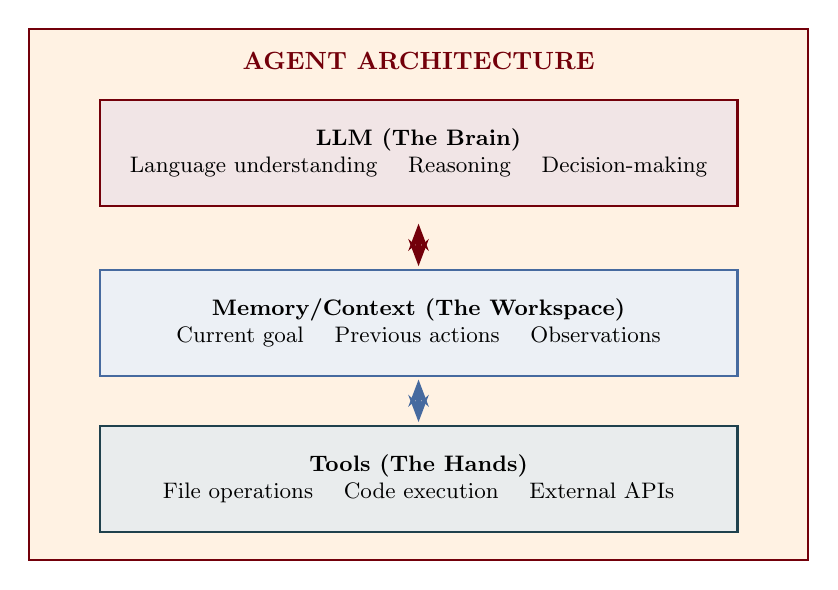
\begin{tikzpicture}[scale=0.9, transform shape]
        % Main container
        \node[draw=UofSCGarnet, thick, minimum width=11cm, minimum height=7.5cm, fill=UofSCSandstorm] (container) at (0,0) {};
        \node[font=\bfseries, text=UofSCGarnet] at (0, 3.3) {AGENT ARCHITECTURE};

        % LLM (Brain)
        \node[component garnet, minimum width=9cm, minimum height=1.5cm] (llm) at (0, 2) {
            \textbf{LLM (The Brain)}\\
            Language understanding \quad Reasoning \quad Decision-making
        };

        % Bidirectional arrow
        \draw[biarrow style, UofSCGarnet, line width=1.5pt] (0, 1) -- (0, 0.4);

        % Memory/Context
        \node[component atlantic, minimum width=9cm, minimum height=1.5cm] (memory) at (0, -0.4) {
            \textbf{Memory/Context (The Workspace)}\\
            Current goal \quad Previous actions \quad Observations
        };

        % Bidirectional arrow
        \draw[biarrow style, UofSCAtlantic, line width=1.5pt] (0, -1.2) -- (0, -1.8);

        % Tools
        \node[component congaree, minimum width=9cm, minimum height=1.5cm] (tools) at (0, -2.6) {
            \textbf{Tools (The Hands)}\\
            File operations \quad Code execution \quad External APIs
        };
    \end{tikzpicture}
\end{document}
